%%%%%%%%%%%%%%%%%%%%%%%%%%%%%%%%%%%%%%%%%%%%%%%%%%%%%%%%%%%%%%%%%%%%5
\chapter{Second Order Circuits and Complex Numbers}
\section{Warm-up}
These questions will warm up some math skills that you'll need to be able to read the chapter. 
\begin{blevel}
Factor: $5e^{x-2y}-4e^{x+2y}$.
\end{blevel}

\begin{alevel}
Solve: $x^2+ 5x - 1 = 0$
\end{alevel}

\begin{blevel}
Solve by completing the square: $x^2+6x-2 = 0$.
\end{blevel}

\begin{clevel}
Derive the quadratic formula for the case when a=1 by completing the square: $x^2+bx+c = 0$.\footnote{You might object. Can't we just use a formula without reinventing it? Well, we can, and do, but we need to balance this will sometimes digging in to see where things come from.}
\end{clevel}

\begin{blevel}
Second order differential equations have terms with second derivatives. Which of the following would be considered second order differential equations?
\begin{description}
\item[Option A] $y'+3y=10$
\item[Option B] $y''+3y'=y$
\item[Option C] $(y')^2+y=10$
\end{description}
\end{blevel}

%%%%%%%%%%%%%%%%%%%%%%%%%%%%%%%%%%%%%%%%%%%%%%%%%%%%%%%%%%%%%%%%%%%%%%%%%
\section{Series RLC Example}
First order circuits, like the RC circuit from the last chapter, lead to first order differential equations. Second order circuits leads to second order differential equations. Not surprisingly, second order systems take a little more thought and technique to analyze. \\
\\
For an example\footnote{All circuits have some inductors and capacitors but many are ignored because they might are small.}, perhaps a wire transmits a changing voltage signal (+5V to 0V) to some computer pin (maybe an Arduino input). See Figure~\ref{F:7EX}.

\begin{figure}[H]
\begin{center}
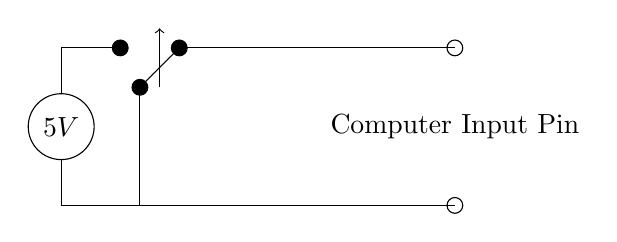
\begin{tikzpicture}
\draw (0,0)--(0,1) node[circle, draw=black,fill=white]{$5V$}--(0,2)
--(.75,2) (1.5,2)--(2,2)--(5,2) (1,0)--(1,1.5);
\draw (1,1.5)--(1.5,2);
\draw (5,2) circle[radius=1 mm];
\draw (5,0) circle[radius=1 mm];
\filldraw (1.5,2) circle[radius=1 mm];
\filldraw (.75,2) circle[radius=1 mm];
\filldraw (1,1.5) circle[radius=1 mm];
\draw [<-] (1.25,2.25)--(1.25,1.5);
\draw (5,0)--(0,0);
\draw node at (5,1) {Computer Input Pin};
\end{tikzpicture}
\caption{Changing voltage signal sent to computer input}
\label{F:7EX}
\end{center}
\end{figure}

The wires have some resistance \footnote{And the source has some internal resistance.} and the whole loop has some inductance. The input to the computer has some capacitance. While the resistance and inductance are not located at any one spot in the wire, they can be modeled as one resistor and one inductor in series, the order of which doesn't matter\footnote{Called a lumped parameter model.}.
\par
Our model for the situation looks like Figure~\ref{F:7EX2}. We now set out to determine the capacitor voltage as a function of time (the voltage that actually reaches the computer input.) 

\begin{figure}[H]
\begin{center}
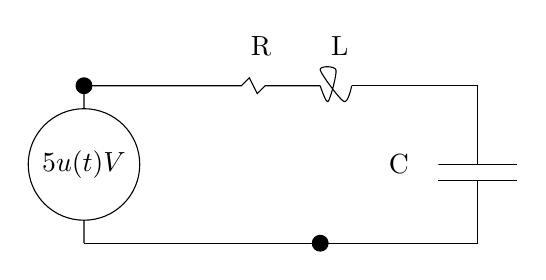
\begin{tikzpicture}
\draw (0,0)--(0,1) node[circle, draw=black,fill=white]{$5u(t) V$}--(0,2)
--(1,2)--(1.5,2)--(2,2)--(2.1,2.1)--(2.2,1.9)--(2.3,2)--(3,2);
\draw plot [smooth] coordinates {(3,2) (3.1,1.8) (3.2,2.2) (3,2.2) (3.3,1.8) (3.4,2)};
\draw (3.4,2)--(5,2)--(5,1)--(4.5,1)--(5.5,1) (4.5,.8)--(5.5,.8) (5,.8)--(5,0)--(0,0);
\filldraw (0,2) circle[radius=1 mm];
\filldraw (3,0) circle[radius=1 mm];
\draw node at (2.25,2.5) {R};
\draw node at (4,1) {C};
\draw node at (3.25,2.5) {L};
\end{tikzpicture}
\caption{Circuit Model, without values.}
\label{F:7EX2}
\end{center}
\end{figure}

Our analysis begins by us creating an initial-conditions table like we did in chapter 6.\linebreak

\begin{clevel}
Fill in the initial condition table, Table~\ref{T:ic}. Assume at time $0_-$ that all currents through and voltages across the R,L and C components are zero. Hint: Which parameters can not change instantly?
\end{clevel}

\par
\begin{table}[H]
\begin{center}
\begin{tabular}{|c|c|c|c|c|} \hline
object	&$I(t=0_{-})$	&$V(t=0_{-})$	&$I(t=0_{+})$	&$V(t=0_{+})$ \\ \hline
5V source&&&& \\ \hline
switch&&&& \\ \hline
R&&&& \\ \hline
L&&&& \\ \hline
C&&&& \\ \hline
\end{tabular}
\caption{Initial condition table.}
\label{T:ic}
\end{center}
\end{table}

Next, use loop analysis for $V_C(t)$ for all times $>$ $t=0_+$.

\begin{align}
5 - IR - L\frac{dI}{dt} - \frac{1}{C}\int{Idt}=0
\end{align}

Integrals \emph{and} derivatives, yuck! We can remove the integrals by taking a derivative of the whole equation w.r.t. time. Then we'll use solving strategy II (see chapter 6).\par

\begin{align}
0 - R\frac{dI}{dt} - L\frac{d^2I}{dt^2} - \frac{I}{C}=0 \notag\\
LI''+RI'+\frac{I}{C}=0 \label{E:7RLC}
\end{align}

The particular solution is easy, it's just 0. To find the homogeneous solution $I_H$, let $I_H=Ae^{mt}$ (no surprise yet). Plugging this back in:

\begin{align}
&Lm^2Ae^{mt}+RmAe^{mt}+\frac{Ae^{mt}}{C}=0 \notag\\
&m^2+\frac{R}{L}m+\frac{1}{LC}=0 \notag\\
m&=\frac{-\frac{R}{L}\pm \sqrt{\frac{R^2}{L^2}-\frac{4}{LC}}}{2} \notag\\
m&=-\frac{R}{2L}\pm \sqrt{\frac{R^2}{4L^2}-\frac{1}{LC}} \label{E:6m} &
\end{align}

Let's pause and get some numbers at this point: suppose R=1, L=1H and C=1F.\footnote{These L and C values are unrealistically big for the computer pin example, but we can easily change them to more realistic values at the end. Just humor me for now.}  Then:\par

\begin{align}
m&=\frac{1}{2}\pm \frac{\sqrt{3}}{2} i &&\text{where i is $\sqrt{-1}$}
\end{align} 

See note \footnote{Many (maybe most) engineering texts write the complex number i as j, which avoid confusing it with the electrical current, i.  This is noble but this book will defer to the common high school math notation and stick to writing $\sqrt{-1}$ as i.}.\\
\\
There are two acceptable values for m, leading to two solutions for $I_C$. Call them $I_{C1}$ and $I_{C2}$. The system is linear so $I_C$ would be any combination of $I_{C1}+I_{C2}$.\footnote{This would not be true if you stumbled into two valid particular solutions, $I_P$.} \par

\begin{align*}
I=I_P+I_H&=0+Ae^{m_1t}+Be^{m_2t} \\
I=I_P+I_H&=Ae^{-\frac{1}{2}t + \frac{\sqrt{3}}{2} it}+Be^{-\frac{1}{2}t - \frac{\sqrt{3}}{2} it} \\
I=e^{-\alpha t}(Ae^{\omega it}+Be^{-\omega it}) &\text{ After letting $\alpha=\frac{1}{2}$ and $\omega=\frac{\sqrt{3}}{2}$}
\end{align*}

\begin{blevel}
What are the units of $\alpha$? What are the units of $\omega$?
\end{blevel}

Because we have two unknowns, A and B, we need two initial conditions to narrow in on a unique solution. We look back at table Table~\ref{T:ic} for guidance and find that:
\begin{align}
I_L(t=0_+)&=0 \label{E:IC1}\\
V_L(t=0_+)&=5V \notag
\end{align}
\par
I'll show two slightly different methods for finding the values of A and B.
\begin{itemize}
\item Method 1: Find the values of A and B while working with complex numbers. Advantage: Builds confidence and comfort working with complex numbers.
\item Method 2: Transform the equation to eliminate the complex numbers and then find the values of A and B. Advantage: Might be more intuitive.
\end{itemize}

%%%%%%%%%%%%%%%%%%%%%%%%%%%%%%%%%%%%%%%%%%%%%%%%%%%%%%%%%%%%%%%%%%%%%%%%%%
\subsection{Method I}
The first initial condition (at time $0^+$) Equation~\eqref{E:IC1} tells us:
\begin{align}
I&=e^{-\alpha t}(Ae^{\omega it}+Be^{-\omega it}) \label{E:6RLC}\\
0&=A+B&&\text{Current is zero when t=0} \notag\\
B&=-A \notag
\end{align}

To use the second initial condition from ~\eqref{E:IC1}, we need determine he voltage across the inductor.\par

\begin{align*}
V_L &= L\frac{dI}{dt}\\
V_L&=-L\alpha e^{-\alpha t}(Ae^{\omega it}+Be^{-\omega it})+
	Le^{-\alpha t}(Ai\omega e^{\omega it}-Bi\omega e^{-\omega it})\\
5&=-L\alpha(A+B)+Li\omega(A-B)\\
5&=Li\omega(2A)\\
A&=\frac{5}{2iL\omega}=-\frac{5i}{2L\omega}\\
B&=\frac{5i}{2L\omega}
\end{align*}

Then, rewriting our solution with the values of A and B,

\begin{align}
I&=e^{-\alpha t}(\frac{-5i}{2L\omega}e^{\omega it}-\frac{-5i}{2L\omega}e^{-\omega it}) \notag\\
I&=-\frac{5i}{2L\omega}e^{-\alpha t}(e^{\omega it}-e^{-\omega it}) \label{E:6M1}
\end{align} 

We're done. Sort of. Equation~\eqref{E:6M1} is correct but suppose we want to graph it or at least ask questions like, ``What is the current after 5 seconds?" How would one even substitute a time of 5 seconds into this equation? \footnote{Some calculators might be able to handle it, but it would seem like magic.}\par
It's time for some background on imaginary numbers.

%%%%%%%%%%%%%%%%%%%%%%%%%%%%%%%%%%%%%%%%%%%%%%%%%%%%%%%%%%%%%%%%%%%%%%
\subsection{Complex Numbers}
In engineering and science, we employ several of types of numbers: integers, rational numbers, real numbers, irrational numbers and now complex numbers. The set of integers is indicated by $\mathbb{Z}$. The set of rational number is called $\mathbb{Q}$. The set of real numbers is called $\mathbb{R}$ and the set of complex numbers is called $\mathbb{C}$.
\par
\begin{alevel}
True or False: $\mathbb{Z} \subset \mathbb{Q}$. The $\subset$ symbol means `subset'. For example $\{2,3\} \subset \{2,3,5\}$, but $\{2,3\} \not\subset \{1,3,5\}$.
\end{alevel}
\begin{alevel}
True or False: $\mathbb{Q} \subset \mathbb{Z}$.
\end{alevel}

Suppose you do something to an integer (or integers), like squaring it, and the result is guaranteed to also an integer, then we say that the integers are \emph{closed} under that operation. For example, the integers are closed under addition because the sum of two integers is guaranteed to be an integer.
\par
\begin{blevel}
Are the integers closed under multiplication? If not, give a counterexample.
\end{blevel}
\begin{blevel}
Are the integers closed under division? If not, give a counterexample.
\end{blevel}
\begin{blevel}
Are the integers closed under subtraction? If not, give a counterexample.
\end{blevel}
\begin{blevel}
Are the whole numbers (integers that are positive or zero) closed under subtraction? If not, give a counterexample.
\end{blevel}
\begin{clevel}
Are the even numbers closed under subtraction? addition? Multiplication? Division? For case answer yes or no and, if no, give a counterexample.
\end{clevel}
\begin{clevel}
Are the rational numbers closed under subtraction? addition? Multiplication? Division? For case answer yes or no and, if no, give a counterexample.
\end{clevel}
\begin{clevel}
Are the rational numbers closed under exponentiation with integer exponents? How about for rational exponents? For case answer yes or no and, if no, give a counterexample.
\end{clevel}
\begin{clevel}
Are the real numbers closed under exponentiation with integer exponents? How about for rational exponents? For case answer yes or no and, if no, give a counterexample.
\end{clevel}

A big deal with complex numbers is that they are closed under addition, subtraction, multiplication, division, and exponentiation with rational and even complex exponents!\\
\\
A complex number, like a 2-D vector, has two independent parts, a real part and what we call an imaginary part. But please note, the so-called imaginary part isn't really \footnote{No pun intended.} any more imaginary than any other number. All numbers are abstract things that only attain as much or little meaning as we assign to them. The number `5' by itself is abstract. 

\begin{alevel}
Let $A = 1+3i$ and $B=2-5i$. Determine (A+B), (A-B), and AB.
\end{alevel}

\begin{alevel}
What is the complex conjugate of 3+5i? Look up what that means if you don't know.
\end{alevel}

\begin{blevel}
What is $i^2$? What is $i^4$? What is $i^5$? What is $i^{502}$? 
\end{blevel}

\begin{clevel}
What is $(\frac{1+i}{\sqrt{2}})^4$? 
\end{clevel}

\begin{clevel}
Consider the matrix $A=\begin{vmatrix} 0&1 \\ -1&0\end{vmatrix}$. What is A*A? What is $A^4$? 
\end{clevel}

Remember rationalizing denominators (removing radicals from a denomonator) in algebra class? We can employ a similar trick to divide complex numbers. For example:\par

\begin{table}[H]
\begin{center}
\begin{tabular}{c|c}
rationalize denomonator&divide complex numbers\\ \hline
$\frac{1+\sqrt{3}}{2+\sqrt{5}}$&	$\frac{1+3i}{2-5i}$\\
$\frac{1+\sqrt{3}}{2+\sqrt{5}}(\frac{2-\sqrt{5}}{2-\sqrt{5}})$&	$\frac{1+3i}{2-5i}(\frac{2+5i}{2+5i})$\\
$=\frac{2-\sqrt{15}+2\sqrt{3}-\sqrt{5}}{-1}$&$=\frac{-13+11i}{29}$\\
$=-2+\sqrt{15}-2\sqrt{3}+\sqrt{5}$&	$=-\frac{13}{29}+\frac{11}{29}i$
\end{tabular}
\end{center}
\end{table}

Picture complex numbers graphically. Real numbers go on a number line. Complex numbers require a plane, as would a 2D vector. Figure~\ref{F:7CN1} shows the complex numbers A = 1+3i (blue) and B = -2+i (red). We traditionally graph the imaginary part on the vertical axis.

\begin{figure}[H]
\begin{center}
\begin{tikzpicture}
\draw[->] (-4,0)--(4,0) node[right] {real};
\draw[->] (0,-1)--(0,4) node[above] {im};
\draw [draw=blue, line width=1mm] [->](0,0)--(1,3);
\draw [draw=red, line width=1mm] [->](0,0)--(-2,1);
\filldraw (1,3) circle[radius=1 mm];
\filldraw (-2,1) circle[radius=1 mm];
\end{tikzpicture}
\caption{Graphical representation of (1+3i) and (-2+i).}
\label{F:7CN1}
\end{center}
\end{figure}

\begin{alevel}What would be the length of the blue arrow in Figure~\ref{F:7CN1}?\end{alevel}

As with vectors (like position or force) we can describe complex numbers with a magnitude and angle, rather than with components (called rectangular form). 

\begin{table}[H]
\begin{center}
\renewcommand{\arraystretch}{1.5}
\begin{tabular}{|c|c|c|} \hline
number	&magnitude	&angle (ccw from East) \\ \hline
1+3i & $\sqrt{10}$	&$71.6^o$\\ \hline
-2+i& $\sqrt{5}$	&$153^o$\\ \hline
\end{tabular}
\caption{Magnitudes and Angles}
\end{center}
\end{table}

Perhaps most surprising\footnote{If you haven't seen it before.} is that complex number can be represented as complex exponentials, called \emph{polar form}.

\begin{table}[H]
\begin{center}
\renewcommand{\arraystretch}{1.5}
\begin{tabular}{|c|c|} \hline
rectangular form	&polar form\\ \hline
1+3i & $\sqrt{10}e^{i71.6^o}$\\ \hline
-2+i& $\sqrt{5}e^{i153^o}$\\ \hline
a+bi&$\sqrt{a^2+b^2}e^{itan^{-1}(\frac{b}{a})}$ \\ \hline
\end{tabular}
\caption{Rectangular and Polar Forms}
\label{T:6EU}
\end{center}
\end{table}

Euler's Formula established the connection between the polar and rectangular forms of a complex number.\footnote{Derived by comparing power series expansions of cos(x), sin(x) and $e^{ix}$. If we don't get to it in class, please try it - it's a beautiful thing.}:
\begin{align}
 e^{ix}=cos(x)+isin(x) \tag{Euler's Formula}
\end{align}

Checking the first row of Table~\ref{T:6EU}.
\begin{align*}
 \sqrt{10}e^{i71.6^o}&=\sqrt{10}(cos(71.6^o)+isin(71.6^o))\\
&=1+3i
\end{align*}

Checking the last row of Table~\ref{T:6EU}.

\begin{align*}
c&=\sqrt{a^2+b^2}e^{itan^{-1}(\frac{b}{a})} &\text{polar form}\\
c&=\sqrt{a^2+b^2}(cos(tan^{-1}(\frac{b}{a}))+isin(tan^{-1}(\frac{b}{a}))) &\text{Used Euler's Equation}\\
c&=\sqrt{a^2+b^2}(\frac{adj}{hyp}+i\frac{opp}{hyp})\\
c&=\sqrt{a^2+b^2}(\frac{a}{\sqrt{a^2+b^2}}+i\frac{b}{\sqrt{a^2+b^2}})&\text{Triangle has sides a and b} \\
c&=a+bi &\rule{1.6ex}{1.6ex}
\end{align*}

\begin{blevel}
Fill in table Table~\ref{T:convert}.
\end{blevel}

\begin{table}[H]
\begin{center}
\begin{tabular}{|c|c|} \hline
rectangular form	&polar form\\ \hline
1+5i & \\ \hline
-2+i& $3e^{i30^o}$\\ \hline
& $3e^{-i30^o}$\\ \hline
2-5i& \\ \hline
& $-2e^{i100^o}$\\ \hline
i& \\ \hline
& $e^{-i90^o}$\\ \hline
\end{tabular}
\caption{Convert rectangular and polar forms.}
\label{T:convert}
\end{center}
\end{table}

For another interesting result, look back at Euler's formula, $e^{ix}=cos(x)+isin(x)$, and write it twice, once with an input of ix and once with an input of -ix. Then add the two versions to each other.
\begin{align}
&e^{ix}&=cos(x)+isin(x) \notag\\
+&e^{-ix}&=cos(-x)+isin(-x)=cos(x)-isin(x) \notag\\
\hline
&e^{ix}+e^{-ix}&=2cos(x)
\end{align}

Therefore, another way to write cos(x) is:
\begin{align}
cos(x)=\frac{e^{ix}+e^{-ix}}{2} \label{E:6COS}
\end{align}

\begin{clevel}
Find another way to write sin(x) by subtracting the two versions instead of adding them.
\end{clevel}

\begin{clevel}
Use equation~\eqref{E:6COS} and its sin(x) equivalent to verify that $sin^2(x)+cos^2(x)=1$.
\end{clevel}


Let's play around with a couple classic examples before we get back to solving our series RLC circuit.

\begin{blevel}
What is: $e^{i\frac{\pi}{2}}$? Here, the angle $\frac{\pi}{2}$ is given in radians.
\end{blevel}

\begin{blevel}
What is: $i^i$? Hint: write one of the i's in complex form. 
\end{blevel}

\begin{clevel}
What does it mean to multiply a number by i? Hint: Consider the number in polar form. Does it change its magnitude? Does it change the angle? What is the difference between multiplying by i and -i?\footnote{We'll come back to this question in the context of currents and voltages.}
\end{clevel}

\subsection{Finish the series RLC problem}
Now, back to our RLC circuit - here's where we left off.

\begin{align}
I&=-\frac{5i}{2L\omega}e^{-\alpha t}(e^{\omega it}-e^{-\omega it})
\end{align} 

Use Euler's Equation to transform those complex exponentials into rectangular form.

\begin{align*}
I&=-\frac{5i}{2L\omega}e^{-\alpha t}(cos(\omega t)+isin(\omega t)-(cos(-\omega t)+isin(-\omega t)))\\
I&=-\frac{5i}{2L\omega}e^{-\alpha t}(cos(\omega t)+isin(\omega t)-(cos(\omega t)-isin(\omega t)))\\
I&=-\frac{5i}{2L\omega}e^{-\alpha t}(2isin(\omega t))\\
I&=\frac{5}{L\omega}e^{-\alpha t}(sin(\omega t))\\
I&=5.77e^{-\frac{1}{2} t}(sin(0.866 t))
\end{align*} 

This last version no longer has any complex parts, so we can readily plug in 5s and get $I(t=5s)=0.439A$ (remember, L=1 H, $\alpha=\frac{1}{2}$, and $\omega=\frac{\sqrt{3}}{2}$).\par 

What does this equation tell us? What would its graph look like? The current is the product of a constant, 5.77 and two other terms: $e^{-\frac{1}{2}t}$ and $sin(0.866t)$. The constant 5.77 just stretches the graph vertically. What remains is a sinuisoid multiplied by a decaying exponential term. 

\begin{figure}[H]
\begin{center}
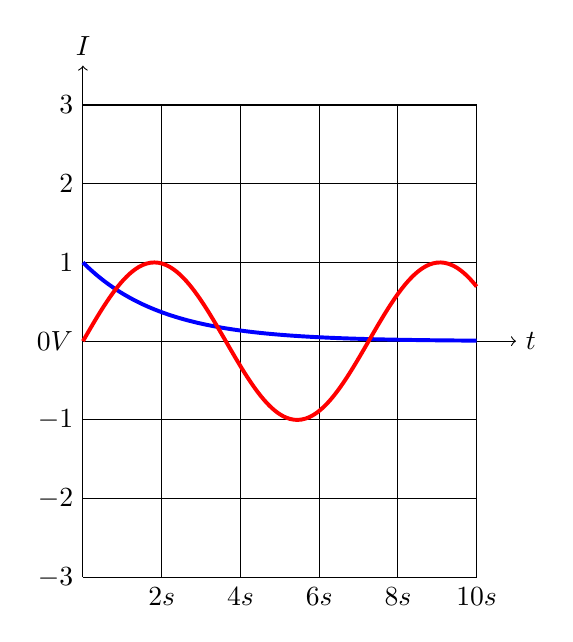
\begin{tikzpicture}
\draw[->] (0,0)--(5.5,0) node[right] {$t$};
\draw[->] (0,-3)--(0,3.5) node[above] {$I$};
\draw (0,0)node[left, line width=0.5] {$0 V$} --(5,0);
\draw (0,-3)node[left] {$-3$} --(5,-3);
\draw (0,-2)node[left] {$-2$} --(5,-2);
\draw (0,-1)node[left] {$-1$} --(5,-1);
\draw (0,1)node[left] {$1$} --(5,1);
\draw (0,2)node[left] {$2$}--(5,2) ;
\draw (0,3)node[left] {$3$}--(5,3) ;
\draw (1,-3)node[below] {$2 s$}--(1,3) ;
\draw (2,-3)node[below] {$4 s$}--(2,3) ;
\draw (3,-3)node[below] {$6 s$}--(3,3) ;
\draw (4,-3)node[below] {$8 s$}--(4,3) ;
\draw (5,-3)node[below] {$10 s$}--(5,3) ;
\draw [draw=blue, line width=.5 mm,smooth, samples=100,domain=0:10,xscale=.5,yscale=1] plot(\x,{exp(-\x/2)});
\draw [draw=red, line width=.5 mm,smooth, samples=100,domain=0:10,xscale=.5,yscale=1] plot(\x,{1*sin(57.29*.866*\x)});
%\draw [draw=blue, line width=.25 mm, dashed] (0,2.5)--(5,2.5);
\end{tikzpicture}
\caption{Exponential term shown in blue. Negative sine term drawn in red.}
\label{F:6RLCG2}
\end{center}
\end{figure}

After multiplying these two parts together, we would then expect an oscillating current with a decreasing amplitude. The oscillating nature of the current is sometimes referred to as ``ringing". Figure~\ref{F:6RLCG} shows a graph of the current as a function of time.

\begin{figure}[H]
\begin{center}
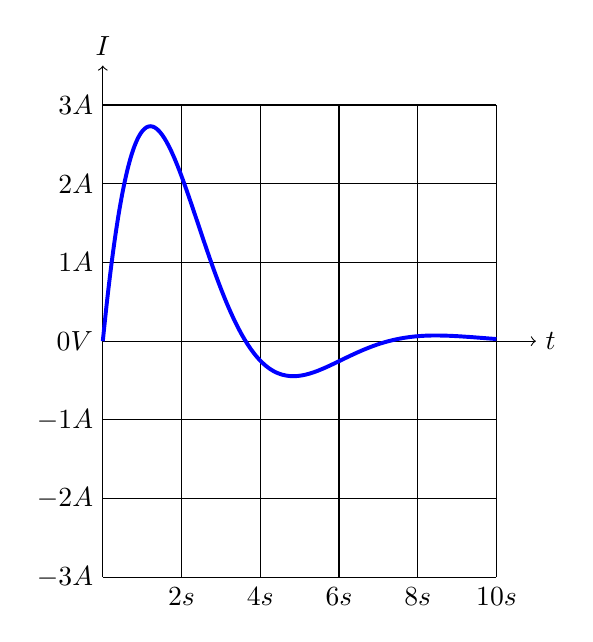
\begin{tikzpicture}
\draw[->] (0,0)--(5.5,0) node[right] {$t$};
\draw[->] (0,-3)--(0,3.5) node[above] {$I$};
\draw (0,0)node[left, line width=0.5] {$0 V$} --(5,0);
\draw (0,-3)node[left] {$-3 A$} --(5,-3);
\draw (0,-2)node[left] {$-2 A$} --(5,-2);
\draw (0,-1)node[left] {$-1 A$} --(5,-1);
\draw (0,1)node[left] {$1 A$} --(5,1);
\draw (0,2)node[left] {$2 A$}--(5,2) ;
\draw (0,3)node[left] {$3 A$}--(5,3) ;
\draw (1,-3)node[below] {$2 s$}--(1,3) ;
\draw (2,-3)node[below] {$4 s$}--(2,3) ;
\draw (3,-3)node[below] {$6 s$}--(3,3) ;
\draw (4,-3)node[below] {$8 s$}--(4,3) ;
\draw (5,-3)node[below] {$10 s$}--(5,3) ;
\draw [draw=blue, line width=.5 mm,smooth, samples=100,domain=0:10,xscale=.5,yscale=1] plot(\x,{5.77*exp(-\x/2)*sin(57.29*.866*\x)});
%\draw [draw=blue, line width=.25 mm, dashed] (0,2.5)--(5,2.5);
\end{tikzpicture}
\caption{I(t) for the series RLC circuit}
\label{F:6RLCG}
\end{center}
\end{figure}

\begin{alevel}
What is the current when the time is 2s?
\end{alevel}

\begin{blevel}
What are the units of the 5.77?
\end{blevel}

\begin{blevel}
Sketch the shape of the graph if $\alpha$ were changed from $-\frac{1}{2}$ to $-\frac{1}{4}$. Sketch the shape of the graph if $\omega$ were changed from $0.866$ $\frac{rad}{s}$ to $2$ $\frac{rad}{s}$.  
\end{blevel}

\begin{clevel}
Find an equation for the voltage across the computer input (modeled as the capacitor) as a function of time? Hint 1: If you know the current onto the capacitor, how can you determine the voltage? Hint 2: If it's an integral relationship, you'll need limits on your integral. What is the voltage across the capacitor when $t=0_+$?
\end{clevel}

Examine the graph of voltage across the capacitor (determined by the previous C-LEVEL problem) shown in Figure~\ref{F:6RLCG}. You'll see that it increases from 0 to 5V as expected, but that it overshoots and wiggles around until it asmptotically reaches 5V. If the resistance is large enough (compared to some combination of the L and C values) then the equation would no longer have a sinusoidal term and therefore the voltage would not overshoot.

\begin{figure}[H]
\begin{center}
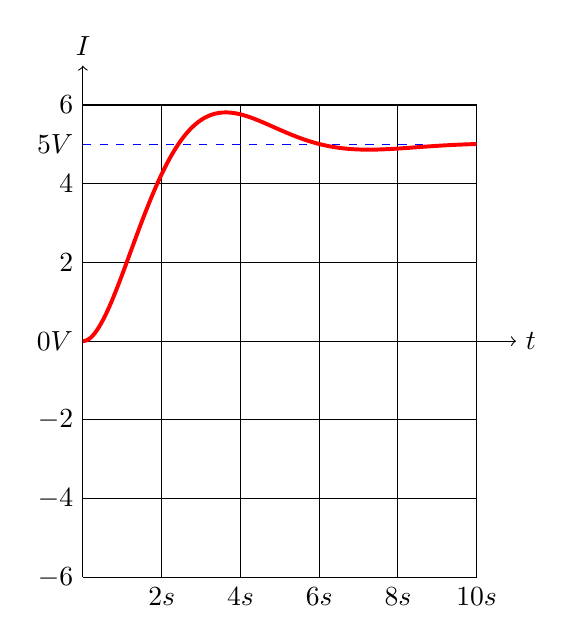
\begin{tikzpicture}
\draw[->] (0,0)--(5.5,0) node[right] {$t$};
\draw[->] (0,-3)--(0,3.5) node[above] {$I$};
\draw (0,0)node[left, line width=0.5] {$0 V$} --(5,0);
\draw (0,-3)node[left] {$-6$} --(5,-3);
\draw (0,-2)node[left] {$-4$} --(5,-2);
\draw (0,-1)node[left] {$-2$} --(5,-1);
\draw (0,1)node[left] {$2$} --(5,1);
\draw (0,2)node[left] {$4$}--(5,2) ;
\draw (0,3)node[left] {$6$}--(5,3) ;
\draw (1,-3)node[below] {$2 s$}--(1,3) ;
\draw (2,-3)node[below] {$4 s$}--(2,3) ;
\draw (3,-3)node[below] {$6 s$}--(3,3) ;
\draw (4,-3)node[below] {$8 s$}--(4,3) ;
\draw (5,-3)node[below] {$10 s$}--(5,3) ;
\draw [dashed, draw=blue] (0,2.5)node[left] {$5V$}--(5,2.5) ;
\draw [draw=red, line width=.5 mm,smooth, samples=100,domain=0:10,xscale=.5,yscale=.5] plot(\x,{5.77*(-0.5*exp(-\x/2)*(sin(57.29*.866*\x)+1.732*cos(57.29*.866*\x))+0.5*1.732)});
%\draw [draw=blue, line width=.25 mm, dashed] (0,2.5)--(5,2.5);
\end{tikzpicture}
\caption{Voltage across the capacitor as a function of time. Note the overshooting.}
\label{F:6RLCG3}
\end{center}
\end{figure}

\begin{alevel}
To the nearest second, what time does the max voltage across the capacitor occur?
\end{alevel}

\begin{clevel}
What is the max voltage across the capacitor (to the nearest hundredth of a Volt)? Hint: Either plug in some values, or it you're brave, use calculus.
\end{clevel}

%%%%%%%%%%%%%%%%%%%%%%%%%%%%%%%%%%%%%%%%%%%%%%%%%%%%%%%%%%%%%%%%%%%%%%%%%%
\subsection{Method II}
Knowing what we now know about complex numbers, we can revisit Equation~\eqref{E:6RLC} and rearrange things differently.\footnote{This ordering might seem more familiar to some of you who are taking a course in differential equations.}

\begin{align}
I=I_H&=e^{-\alpha t}(Ae^{\omega it}+Be^{-\omega it}) \tag{where $\alpha=\frac{1}{2}$ and $\omega=\frac{\sqrt{3}}{2}$}
\end{align}

This time, employ Euler's equation immediately and then combine terms.

\begin{align}
I&=e^{-\alpha t}(A(cos(\omega t)+isin(\omega t))+B(cos(-\omega t)+isin(-\omega t))) &\text{Euler}\notag\\
I&=e^{-\alpha t}(Acos(\omega t)+Aisin(\omega t)+Bcos(\omega t)-Bisin(\omega t))) \notag\\
&\rightarrow \text{Used trig identities}\\
I&=e^{-\alpha t}((A+B)cos(\omega t)+(Ai-Bi)sin(\omega t)) \notag\\
&\rightarrow\text{Let (A+B)=C and (Ai+Bi)=D} \notag\\
I&=e^{-\alpha t}(Ccos(\omega t)+Dsin(\omega t)) \label{E:M2} 
\end{align}

Some just give up on understanding and try to memorize this formula. Resist the temptation. \par

We still need to employ initial conditions (Equation ~\eqref{E:IC1} into ~\eqref{E:M2}) to find the values of C and D.

\begin{align*}
I&=e^{-\alpha t}(Ccos(\omega t)+Dsin(\omega t))  \\
0&=1(C+D(0)) &&\text{Used $I(0)=0$}\\
C&=0
\end{align*}

To use the other initial condition ($V_L(0)=0$), we first determine the voltage across the inductor (~\eqref{E:M2}).\par

\begin{align}
V_L&=L\frac{dI}{dt} \notag \\
V_L&=L\frac{d(e^{-\alpha t}(Dsin(\omega t)))}{dt} \notag \\
V_L&=-L\alpha(e^{-\alpha t}(Dsin(\omega t)))+Le^{-\alpha t}D\omega cos(\omega t) \notag \\
5 &= LD\omega \notag\\
D &= \frac{5}{L\omega}
\end{align}

The current is:
\begin{align}
I&=5.77e^{-\frac{1}{2} t}(sin(0.866 t)) \label{E:7RLCSOL}
\end{align}

\begin{alevel}
What are the units of the 0.866?
\end{alevel}

\begin{dlevel}
How much time will pass until the voltage across the capacitor never deviates again by more than 10\% from 5V (4.5 to 5.5V)?
\end{dlevel}

\begin{clevel}
Repeat the analysis to determine the equation for the current, $I_L(t)$, and the voltage across the capacitor, but where value of R is changed to 0.5 Ohms instead of 1 Ohm. 
\end{clevel}

If the value of R were changed from 1 to 3 Ohms, the oscillatory behavior would stop (no overshooting). The next problems explore this a little.

\begin{clevel}
If value of R were 3 Ohms instead of 1 Ohm, determine the new m-values for the complementary solution, $I_C$ (also called the homogeneous solution, $I_H$).
\end{clevel}

\begin{clevel}
If value of R were 3 Ohms instead of 1 Ohm, determine a new equation for $I_C$ ($I_P$ is still zero). Plug in the same initial conditions as before and determine any unknown constants. Hint: you'll need to do a little algebra. Just follow where the math takes you.
\end{clevel}

\begin{clevel}
In terms of L and C, what is the precise value of R that will be the cut-off between ringing and not ringing?
\end{clevel}

%%%%%%%%%%%%%%%%%%%%%%%%%%%%%%%%%%%%%%%%%%%%%%%%%%%%%%%%%%%%%%%%%%%%%
\section{Mechanical Analog to Second Order Circuit}
An RC circuit behaves like a massless object on a spring (with drag). Is there a mechanical system that behaves as a second order circuit like the series RLC circuit that we studied here? Yes, just include the mass of the object (you know you were eager to include it anyway:) ) 

\begin{figure}[H]
\begin{center}
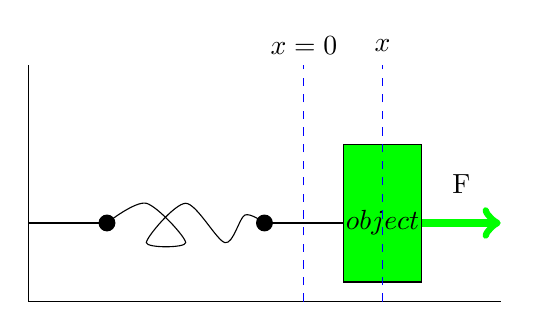
\begin{tikzpicture}
\draw (0,0)--(0,3) (0,0)--(6,0);
\draw [draw=black, fill=green] (4,.25) rectangle (5,2);
\filldraw (3,1) circle[radius=1 mm];
\draw plot [smooth] coordinates {(1,1) (1.5,1.25) (2,.75) (1.5,.75) (2,1.25) (2.5,.75) (2.75,1.1) (3,1)};
\filldraw (1,1) circle[radius=1 mm];
\draw node at (4.5,1) {$object$};
\draw (3,1)--(4,1) (0,1)--(1,1);
\draw node at (4.5,3.25) {$x$};
\draw node at (3.5,3.25) {$x=0$};
\draw [dashed, draw=blue] (4.5,0)--(4.5,3) (3.5,0)--(3.5,3);
\draw [draw=green, line width=1 mm] [->] (5,1)--(6,1);
\draw [draw=green] node at (5.5,1.5) {F};
\end{tikzpicture}
\caption{Mechanical Analog to RC circuit. Mass on spring with frictional drag.}
\label{F:7RCM}
\end{center}
\end{figure}

We suddenly applying a constant force (shown in green) to the mass as illustrated in Figure~\ref{F:7RCM}. Set the constant force to 5N, the mass to 7 kg, the spring constant to 2 N/m and the drag coefficient to b=3 Ns/m. Writing out F=ma:

\begin{align}
F_T=ma=m\frac{d^2x}{dt^2}\notag\\
F-kx-bv=m\frac{d^2x}{dt^2}\notag\\
5-2x-3\frac{dx}{dt}=7\frac{d^2x}{dt^2}\notag\\
7\frac{d^2x}{dt^2}+3\frac{dx}{dt}+2x=5 \\
7\frac{d^2v}{dt^2}+3\frac{dv}{dt}+2v=0 \label{E:7MA}
\end{align}

Compare this with equation~\eqref{E:7RLC} and hopefully you can see some similarities.

\begin{alevel}
What are the units of the `3'?
\end{alevel}

\begin{blevel}
Identify a circuit that would yield exactly Equation~\eqref{E:7MA}.
\end{blevel}

\begin{clevel}
Find the homogenous solution to Equation~\eqref{E:7MA}. Are you m-values real or imaginary? What does them being real or imaginary tell you about the physical situation?
\end{clevel}

\begin{clevel}
Fully solve Equation~\eqref{E:7MA} for x(t).
\end{clevel}

\begin{dlevel}
Determine a mechanical problem that results in exactly equation~\eqref{E:7RLCSOL}.
\end{dlevel}
%%%%%%%%%%%%%%%%%%%%%%%%%%%%%%%%%%%%%%%%%%%%%%%%%%%%%%%%%%%%%%%%%%%%%%%%%%
\section{Another second order circuit example}
Consider a different circuit shown in Figure~\ref{F:7EX2}, where $R_1=4\Omega$,$R_2=2\Omega$,$C=2F$,$L=3H$. Start with nodal analysis because the circuit has three loops but only one unknown node voltage.

\begin{figure}[H]
\begin{center}
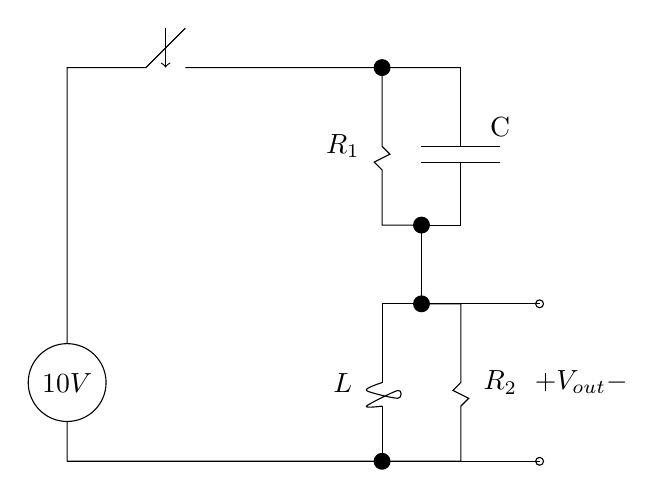
\begin{tikzpicture}
\draw (0,0)--(0,1) node[circle, draw=black,fill=white]{$10V$}--(0,5)
--(1,5)--(1.5,5.5) (1.5,5)--(2,5)--(5,5);
\draw [<-] (1.25,5)--(1.25,5.5);
\filldraw (4,5) circle[radius=1 mm];
\filldraw (4.5,3) circle[radius=1 mm];
\draw (4.5,3)--(4.5,2);
\filldraw (4.5,2) circle[radius=1 mm];
\draw (4,5)--(4,4)--(4.1,3.9)--(3.9,3.8)--(4,3.7)--(4,3)--(4.5,3);
\draw node at (3.5,4) {$R_1$};
\draw (5,5)--(5,4)--(5.5,4)--(4.5,4) (4.5,3.8)--(5.5,3.8) (5,3.8)--(5,3)--(4.5,3);
\draw node at (5.5,4.25) {C};
\draw (4.5,2)--(4,2)--(4,1) (4,.7)--(4,0);
\draw plot [smooth] coordinates {(4,1) (3.8,0.9) (4.2,.8) (4.2,.9) (3.8,.7) (4,.7)};
\draw (4.5,2)--(5,2)--(5,1)--(4.9,.9)--(5.1,.8)--(5,.7)--(5,0)--(0,0);
\draw node at (5.5,1) {$R_2$};
\draw node at (3.5,1) {$L$};
\filldraw (4,0) circle[radius=1 mm];
\draw (4.5,2)--(6,2) (4.5,0)--(6,0);
\draw (6,2) circle[draw=black,radius=.5 mm];
\draw (6,0) circle[draw=black,radius=.5 mm];
\draw node at (6.5,1) {$\begin{matrix}+\\V_{out}\\-\end{matrix}$};
\end{tikzpicture}
\caption{Second Example}
\label{F:7EX2}
\end{center}
\end{figure}

Begin by determining the initial conditions. We need to make several observations in order to proceed.
\begin{itemize}
\item Before the switch closes, we assume that voltages and currents are not changing. Ask yourself, what is the voltage across a capacitor if the current is not changing?
\item Fill in all parameters for time $0_-$
\item For the instant after the switch closes, identify the values that can not change instantly.
\item Fill in the rest of the table.
\end{itemize}

\begin{clevel}
Fill in the initial condition table, Table~\ref{T:ic2}.
\end{clevel}

\par
\begin{table}[H]
\begin{center}
\begin{tabular}{|c|c|c|c|c|} \hline
object	&$I(t=0_{-})$	&$V(t=0_{-})$	&$I(t=0_{+})$	&$V(t=0_{+})$ \\ \hline
5V source&&&& \\ \hline
switch&&&& \\ \hline
$R_1$&&&& \\ \hline
$R_2$&&&& \\ \hline
L&&&& \\ \hline
C&&&& \\ \hline
\end{tabular}
\caption{Initial condition table.}
\label{T:ic2}
\end{center}
\end{table}

\begin{blevel}
Write a node equation for the node ($V_{out}$) after the switch has closed.
\end{blevel}

\begin{clevel}
Solve your node equation for $V_{out}(t)$. Use whichever method you prefer, but I recommend both methods.Use initial conditions to determine any unknowns. Determine $V_{out}$ when t=0.5 seconds.
\end{clevel}

\begin{blevel}
Based on your answer, does the voltage oscillate?
\end{blevel}

\begin{blevel}
Based on your answer, what is $V_{out}(t \rightarrow \infty)$?
\end{blevel}

